\documentclass[11pt,a4paper]{article}
%%%%%%%%%%%%%%%%%%%%%%%%%%%%%%%%%%%%%%%%%%%%%%%%%%%%%%%%
%                      PACKAGES                        %
%%%%%%%%%%%%%%%%%%%%%%%%%%%%%%%%%%%%%%%%%%%%%%%%%%%%%%%%

\usepackage[utf8]{inputenc}
\usepackage{graphicx} % Allows you to insert figures
\usepackage[export]{adjustbox}
\usepackage{booktabs}
\usepackage{amsmath} % Allows you to do equations
\usepackage{helvet}
\usepackage{hyperref}
\renewcommand{\familydefault}{\sfdefault}
\usepackage[a4paper, total={6.5in, 9.5in}]{geometry} % Formats the paper size, orientation, and margins
\linespread{1.1} % about 1.5 spacing in Word
\setlength{\parindent}{0pt} % no paragraph indents
\setlength{\parskip}{1em} % paragraphs separated by one line
\usepackage{listings}
\usepackage{enumitem}
\usepackage{xcolor}
\usepackage{hyperref}
\usepackage{pmboxdraw}
\usepackage{dirtree}

\hypersetup{
	colorlinks=true,
	urlcolor=cyan,
	linktoc=none,
}
\usepackage{fancyhdr}
\usepackage{float}

\pagestyle{fancy}
\fancyhead[L,C,R]{}
\fancyfoot[L]{Blix - AI Photo Editor}
\fancyfoot[C]{}
\fancyfoot[R]{\textbf{\thepage}}
\renewcommand{\headrulewidth}{0pt}
\renewcommand{\footrulewidth}{0.5pt}

\definecolor{codegreen}{rgb}{0,0.6,0}
\definecolor{codegray}{rgb}{0.5,0.5,0.5}
\definecolor{codepurple}{rgb}{0.58,0,0.82}
\definecolor{backcolour}{rgb}{0.95,0.95,0.92}

\usepackage{listings}

% Define TypeScript language style
\lstdefinelanguage{TypeScript}{
  keywords=[1]{class, constructor, let},
  keywordstyle=[1]\bfseries,
  keywords=[2]{string},
  keywordstyle=[2]\color{blue},
  sensitive=true,
  morestring=[b]',
  morestring=[b]"
}


\lstdefinestyle{mystyle}{
backgroundcolor=\color{backcolour},
commentstyle=\color{codegreen},
keywordstyle=\color{magenta},
numberstyle=\tiny\color{codegray},
stringstyle=\color{codepurple},
basicstyle=\ttfamily\footnotesize,
breakatwhitespace=false,
breaklines=true,
keepspaces=true,
numbers=left,
numbersep=5pt,
showspaces=false,
showstringspaces=false,
showtabs=false,
tabsize=2,
}

\lstset{style=mystyle}
\def\code#1{\texttt{#1}}

%%%%%%%%%%%%%%%%%%%%%%%%%%%%%%%%%%%%%%%%%%%%%%%%%%%%%%%%
%            TITLE PAGE & TABLE OF CONTENTS            %
%%%%%%%%%%%%%%%%%%%%%%%%%%%%%%%%%%%%%%%%%%%%%%%%%%%%%%%%

\begin{document}

\begin{titlepage}
	\centering
    % \includegraphics[width=0.5\textwidth]{your_logo.png}\par\vspace{1cm}
    {\scshape\LARGE Testing Policy V1\par}
    \vspace{1.5cm}
    {\huge\bfseries Blix - AI Photo Editor\par}
    \vspace{2.5cm}
    \begin{figure}[h]
        \centering % center the image
        \includegraphics[width=0.5\textwidth]{../pics/blix.png}
    \end{figure}
    \vspace{2.5cm}
    {\Large\itshape The Spanish Inquisition\par}

    \vfill
    {\large \today\par}
\end{titlepage}

\tableofcontents
\pagebreak

%%%%%%%%%%%%%%%%%%%%%%%%%%%%%%%%%%%%%%%%%%%%%%%%%%%%%%%%
%                MAIN DOCUMENT CONTENT                 %
%%%%%%%%%%%%%%%%%%%%%%%%%%%%%%%%%%%%%%%%%%%%%%%%%%%%%%%%

\addcontentsline{toc}{section}{Introduction}
\section*{Introduction}

Introducing Blix: An Advanced AI Photo Editor

Welcome to Blix, an innovative and sophisticated AI-powered photo editing application. Blix sets itself apart by providing users with a seamless editing experience through a powerful and 
intuitive interface, reminiscent of a digital blender. This user manual will guide you through the features and functionalities of Blix, enabling you to harness the full potential of 
this cutting-edge editing tool.

Blix caters to users of all levels, from amateur photographers to seasoned professionals, by streamlining the editing process and eliminating the need 
for extensive knowledge of complex editing software. By presenting a visual graph-based interface, akin to a blender, Blix enables effortless mixing and matching of diverse editing effects.

As a user, you gain access to a vast array of editing possibilities. Whether you wish to apply filters, fine-tune brightness and contrast, or add artistic effects such as vignettes or vintage tones, Blix provides an extensive selection of editing options. Each editing choice is represented as a node within the graph, allowing for seamless connectivity and the creation of custom editing flows tailored to your preferences.

What truly sets Blix apart is its integration of cutting-edge AI technology. Through Blix, you can engage with an AI assistant that enhances your editing journey. 
By sending prompts to the AI, you unlock a world of possibilities. The AI assistant can recommend specific edits, suggest optimal adjustments, or even manipulate the graph on your behalf, 
all based on your unique preferences and the desired outcome.

In summary, Blix is an advanced AI photo editor that empowers users to elevate their photography with ease and finesse. Its intuitive graph-based interface, extensive editing options, 
and integration with an AI assistant create a harmonious environment for realizing your creative vision. This user manual will serve as your comprehensive guide, enabling you 
to navigate the features of Blix and unlock the full potential of your photo editing capabilities.
\pagebreak


\addcontentsline{toc}{section}{General Testing Characteristics}
\section*{General Testing Characteristics}   

During the continued developement of Blix, we have made use of a variety of testing techniques. These techniques include unit testing, integration testing, and end to end testing.
In order to facilitate the testing process, we have made use of a variety of tools. These tools include Jest, playwright, codecov and github workflows. 
These tools have been used to test the functionality of the application, automate the testing process, and ensure that the application is properly covered by tests.


\addcontentsline{toc}{subsection}{Unit Testing}
\subsection*{Unit Testing}

Unit testing is a software testing method by which individual units of source code are tested to determine whether they are working as intended.
Blix has been extensively tested using unit testing. This has been done using the Jest framework. 

Jest is a JavaScript testing framework designed to ensure correctness of any JavaScript/Typescript codebase.
All of the core functionality of Blix has been unit tested. This includes the functionality of the graph, the AI assistant, the plugins, and the user interface, ensuring that each function 
executes correctly at an atomic level in isolation. 

\addcontentsline{toc}{subsection}{Integration Testing}
\subsection*{Integration Testing}

Integration testing is the phase in software testing in which individual software modules are combined and tested as a group.
In the various subsystems of Blix, integration tests have been used to ensure that the subsystems are working together as intended. This has also been done using the Jest framework.
Each subsystem in their entirety as well as the subsystems communicating with each other have been tested, ensuring that all interactions between systems and the travel of data between systems is correct.

Minimal or no mocking is used for Integration testing as we want to test the actual functionality of the application such that communication and interaction between systems is tested, and
not the atomic operations of each system. Mocks are mainly used for integration tests when testing a subsystem that uses an external resource such as an api request. 


\subsubsection*{JEST}
\addcontentsline{toc}{subsubsection}{JEST}

The reason why we chose Jest for our unit and integration testing is because it is a very popular testing framework that has TypeScript support and meshes easily
with the rollup of our electron app. Jest is easy to use and has a lot of functionality that makes testing easier, such as mocking and code coverage.

Furthermore due to the popularity of Jest, there is a lot of documentation and support for it, which makes it easy to use and learn, which was essential considering our 
lack of experience with testing frameworks

\addcontentsline{toc}{subsection}{End to End Testing}
\subsection*{End to End Testing}

End-to-end testing is a technique used to test whether the flow of an application is performing as designed from start to finish. The purpose of carrying out end-to-end tests is to identify system dependencies and to ensure that the right information is passed between various system components and systems.
Blix has multiple end to end tests that test the correct functionality of the application as a whole. These tests are done using the playwright framework. Playwright is a Node.js library to automate Chromium, Firefox and WebKit with a single API. 

These end to end tests either start in the backend or the frontend, and ensure that all the systems execute according to specification untill the request or result finally reaches the other end of the stack.
End to end testing is inherently slow and all-encompasing, and therefore there are fewer tests for it. These tests are done to ensure that the application is working as a whole, and that all the systems are communicating correctly.


\subsubsection*{Playwright}

Playwright was chosen for the end-to-end tests due to its support for multiple platforms such as Windows, Linux and MacOS and has built-in 
integrations to interact with jest, our testing framework of choice for unit and integration testing. 

Furthermore playwright is relatively easy to use and has a lot of documentation and support,
due to its popularity, which makes it easy to learn and use.

\addcontentsline{toc}{subsection}{CICD}
\subsection*{CICD}

For the purposes of testing, we have made use of github workflows. Github workflows are a feature of github that allow for the automation of tasks.
We have made use of github workflows to automate the testing process. 

This is done by running the tests on every pull request, and on every push
to the main branch. This ensures that the application is always tested before any changes are merged into the main branch.

The tests that are automated for this purpose consist of : 
\begin{itemize}
  \item Unit tests
  \item Integration tests
  \item End to end tests
  \item Building the application
  \item Linting the application
  \item Secret protection
  \item Code coverage
\end{itemize}

\begin{figure}[htbp]
  \centering
  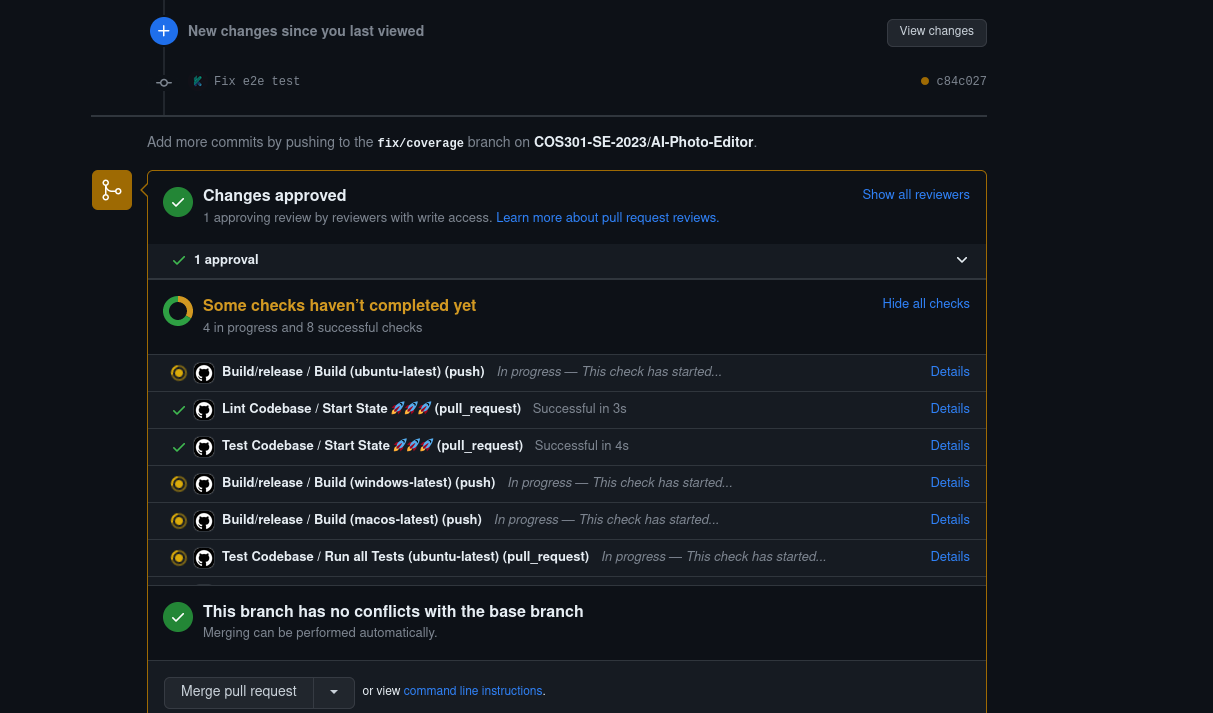
\includegraphics[width=0.95\textwidth]{../pics/cicd.png}
  \caption{Continuous Integration and Continuous Deployment (CI/CD) Pipeline}
\end{figure}

The reason why we chose github workflows for our cicd pipeline is because it enables us to build and test our app for Windows,Linux and MacOS without having to set up a local environment for each of these operating systems.
This is done by using the github hosted runners. These runners are virtual machines that run the github workflows. 

The github hosted runners are free to use for open source projects, and therefore we can use them for our project,
allowing us to cut costs and save time. Furthermore github workflows are easy to set up and use, and are integrated with github, allowing us to easily automate our testing process.

For a more in depth view of our cicd pipeline, please refer to the following link : \url{https://github.com/COS301-SE-2023/AI-Photo-Editor/actions}

\addcontentsline{toc}{subsection}{Software Quality Assurance}
\subsection*{Software Quality Assurance}

The software requirements specification outlines quality criteria that must be assessed, measured, and validated for compliance within the project. 
These criteria are summarized briefly here and elaborated upon in dedicated sections.

\begin{enumerate}[label*=\arabic*.]
  \item Performance
  \item Customizability/Extensibility
  \item Usability
  \item Security
  \item Compatibility
  \item Reliability
\end{enumerate}


\end{document}